\section{Příklad filtrační maska}
Na obrázku je výřez obrazové funkce. Tučně je ohraničeno okolí, ve kterém se má vypočítat filtrovaná hodnota, 
tj. filtrační maska. Vypočtěte filtrované hodnoty při vyhlazování
\begin{enumerate}[(a)]
    \item obyčejným průměrováním,
    \item mediánovou filtrací
\end{enumerate}  
pro právě zpracovávaný pixel ležící ve středu filtrační masky.

\begin{figure}[H]
    \centering
    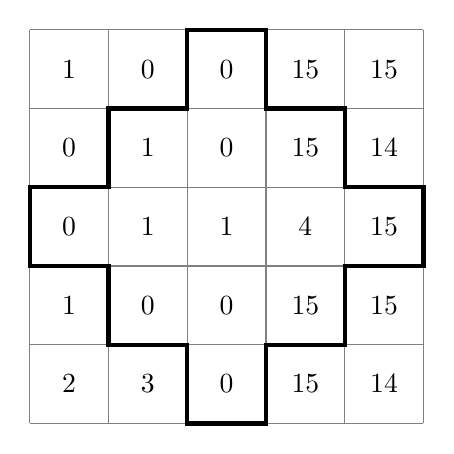
\begin{tikzpicture}[
        cell/.style={
            rectangle,
            minimum size=1cm,
            anchor=center
        }
    ]

    % (0,0) at left down corner
    \draw[step=1cm, gray, thin] (0,0) grid (5,5);

    % (x, y, value)
    \def\tabledata{
        {0/4/1}, {1/4/0}, {2/4/0}, {3/4/15}, {4/4/15},
        {0/3/0}, {1/3/1}, {2/3/0}, {3/3/15}, {4/3/14},
        {0/2/0}, {1/2/1}, {2/2/1}, {3/2/4},  {4/2/15},
        {0/1/1}, {1/1/0}, {2/1/0}, {3/1/15}, {4/1/15},
        {0/0/2}, {1/0/3}, {2/0/0}, {3/0/15}, {4/0/14},
    }

    % add numbers to cells
    \foreach \x/\y/\value in \tabledata {
        \node[cell] at (\x.5, \y.5) {\value};
    }

    % --- bold lines ---
    \draw[line width=1.5pt] 
        (2,5) -- (3,5) -- (3,4) -- (4,4) -- (4,3) -- (5,3) -- (5,2) -- (4,2) -- 
        (4,1) -- (3,1) -- (3,0) -- (2,0) -- (2,1) -- (1,1) --  (1,2) -- (0,2) -- (0,3) -- (1,3) -- 
        (1,4) -- (2,4) -- cycle;

    \end{tikzpicture}
    \caption{Výřez obrazové funkce}
\end{figure}